\documentclass{VUMIFPSbakalaurinis}
\usepackage{algorithmicx}
\usepackage{algorithm}
\usepackage{algpseudocode}
\usepackage{amsfonts}
\usepackage{amsmath}
\usepackage{bm}
\usepackage{caption}
\usepackage{color}
\usepackage{float}
\usepackage{graphicx}
\usepackage{listings}
\usepackage{subfig}
\usepackage{url}
\usepackage{wrapfig}
\usepackage[table,xcdraw]{xcolor}
\usepackage[backend=biber]{biblatex}
\usepackage{enumitem}\setlist{nosep}

% Titulinio aprašas
\university{Vilniaus universitetas}
\faculty{Informatikos institutas}
\department{Programų sistemos}
%\papertype{Bakalauro darbas}
\papertype{Bakalauro baigiamojo darbo planas}
\title{Sustiprinto mokymosi taikymas žaidimo agento valdymo programos kūrimui}
\titleineng{Application of reinforcement learning to the software development for game agent management}
\author{Jokūbas Rusakevičius}
\supervisor{<reikia parašyti pareigas> Virginijus Marcinkevičius}
\reviewer{}
\date{Vilnius – \the\year}

% Nustatymai
\setmainfont[ItalicFont 	= Palem3.2-it.ttf,
			BoldItalicFont	=Palem3.2-bi.ttf,
			BoldFont		=Palem3.2-bd.ttf]
			{Palem3.2-nm.ttf}

\begin{document}
\maketitle

\setcounter{page}{2}


\subsectionnonum{Tyrimo objektas ir aktualumas}



\subsectionnonum{Darbo tikslas, keliami uždavyniai ir laukiami rezultatai}
Šio darbo \textbf{tikslas} - išanalizavus populiariausius sustiprinto mokymosi algoritmus, pritaikyti labiausiai tinkamą algoritmą parinktai eksperimentiniai aplinkai bei pagerinti gaunamus rezultatus pritaikius agento mokymosi gerinimo principus.\par

Darbui iškelti \textbf{uždaviniai}:\par

\begin{enumerate}
	\item Paruošti eksperimentinę aplinką ir agentą.
	\item Apmokyti agentą.
	\item Palyginti gaunamą agento efektyvumą atliekant aplinkoje realizuotą užduotį, keičiant aplinkos bei agento mokymosi kriterijus.
	\item Pateikti rekomendacijas agento apmokymui parinktoje aplinkoje.
\end{enumerate}

Darbo metu laukiami \textbf{rezultatai}:

\begin{enumerate}
	\item Paruošta eksperimentinė aplinka ir agentas.
	\item Agentas yra apmokytas.
	\item Pakeisti aplinkos ir agento mokymosi kriterijai, palyginti gaunami rezultatai ir taip pasiektas geriausias užduoties atlikimas.
	\item Pateiktos rekomendacijos agento apmokymui parinktoje aplinkoje.
\end{enumerate}

\subsectionnonum{Tyrimo metodas} 
Darbui atlikti bus naudojami šie tyrimo metodai:

\begin{enumerate}
	\item \textbf{Mokslinės lteratūros analizė}.
	\item \textbf{Eksperimetas}.
	\subitem \textbf{Kiekybinis metodas} - apmokyti pirminius agentus, stebėti jų elgseną. Atliekamas, su keliais skirtingais kriterijais ir ieškoma tinkamiausio bei daugiausiai žadančio pradinio rezultato eksperimentui.
	\subitem \textbf{Kokybinis metodas} - su gautais pradiniais agentais bei jų mokymosi kriterijais atliekamos gilesnės kriterijų bei agento mokymosi parametrų manipuliacijos bei stebimi gaunamų rezultatų pakitimai.
	\item \textbf{Gautų duomenų ir rezultatų analizė}.
\end{enumerate}

\subsectionnonum{Numatomas darbo atlikimo procesas}
Darbo procesas susidės iš kelių skirtingų dalių:

\begin{enumerate}
	\item Visų pirma, eksperimentui atlikti bus paruošta eksperimentinė aplinka.
	\item Agento paruošimas bus atliekamas pasirenkant pradinius, neutralius mokymosi kriterijus.
	\item Atliekamas pirminis agento apmokymas, skirtas eksperimento bazei gauti bei įsitikinto aplinkos ir agento tarpusavio veikla. 
	\item Pradėjus pagrindinę eksperimento dalį bus ieškoma ir eksperimentuojama su metodais, kuriuos pritaikius būtų gaunami geresni nei aukščiau gaunami rezultatai.
	\item Galutinė visų atliktų tyrimų ir gautų rezultatų analizė.
	\item Pateikiamos rekomendacijos, kaip pagerinti agento apmokymą parinktai aplinkai ir jos keliamoms problemoms bei uždaviniams.
\end{enumerate}


\subsectionnonum{Darbui aktualūs literatūros šaltiniai}

\begin{enumerate}
	\item \textbf{\cite{asap}} - Standfordo Universiteto straipsnis apie laiko intervalu fiksuojamus duomenis bei jų išlyginimą, padaryma lengviau skaitomais. Straipsnyje tai vadinama ASAP, analitiniu operatoriumi, kuris automatiškai išlygina įrašų rinkinį, taip padidinant analizuojamų duomenų gautų rezultatų tikslumą, bei sumažinant skaičiavimams reikalingą greitį.
\end{enumerate}




%\section{Medžiagos darbo tema dėstymo skyriai}
%Medžiagos darbo tema dėstymo skyriuose išsamiai pateikiamos nagrinėjamos temos detalės: pradiniai duomenys, jų analizės ir apdorojimo metodai, sprendimų įgyvendinimas, gautų rezultatų apibendrinimas.

%Medžiaga turi būti dėstoma aiškiai, pateikiant argumentus. Tekste dėstomas trečiuoju asmeniu, t.y. rašoma ne „aš manau“, bet „autorius mano“, „autoriaus nuomone“. Reikėtų vengti informacijos nesuteikiančių frazių, pvz., „...kaip jau buvo minėta...“, „...kaip visiems žinoma...“ ir pan., vengti grožinės literatūros ar publicistinio stiliaus, gausių metaforų ar panašių meninės išraiškos priemonių. Skyriai gali turėti poskyrius ir smulkesnes sudėtines dalis, kaip punktus ir papunkčius.

%\subsection{Poskyris}
%Citavimo pavyzdžiai: cituojamas vienas šaltinis \cite{PvzStraipsnLt}; cituojami keli šaltiniai \cite{PvzStraipsnEn, PvzKonfLt, PvzKonfEn, PvzKnygLt, PvzKnygEn, PvzElPubLt, PvzElPubEn, PvzMagistrLt, PvzPhdEn}.

%\subsubsection{Skirsnis}
%\subsubsubsection{Straipsnis}
%\subsubsection{Skirsnis}
%\section{Skyrius}
%\subsection{Poskyris}
%\subsection{Poskyris}

%\sectionnonum{Rezultatai ir išvados}
%Rezultatų ir išvadų dalyje išdėstomi pagrindiniai darbo rezultatai (kažkas išanalizuota, kažkas sukurta, kažkas įdiegta), toliau pateikiamos išvados (daromi nagrinėtų problemų sprendimo metodų palyginimai, siūlomos rekomendacijos, akcentuojamos naujovės). Rezultatai ir išvados pateikiami sunumeruotų (gali būti hierarchiniai) sąrašų pavidalu. Darbo rezultatai turi atitikti darbo tikslą.

\printbibliography[heading=bibintoc]  % Šaltinių sąraše nurodoma panaudota
% literatūra, kitokie šaltiniai. Abėcėlės tvarka išdėstomi darbe panaudotų
% (cituotų, perfrazuotų ar bent paminėtų) mokslo leidinių, kitokių publikacijų
% bibliografiniai aprašai. Šaltinių sąrašas spausdinamas iš naujo puslapio.
% Aprašai pateikiami netransliteruoti. Šaltinių sąraše negali būti tokių
% šaltinių, kurie nebuvo paminėti tekste. Šaltinių sąraše rekomenduojame
% necituoti savo kursinio darbo, nes tai nėra oficialus literatūros šaltinis.
% Jei tokių nuorodų reikia, pateikti jas tekste.

% \sectionnonum{Sąvokų apibrėžimai}
%\sectionnonum{Santrumpos}
%Sąvokų apibrėžimai ir santrumpų sąrašas sudaromas tada, kai darbo tekste vartojami specialūs paaiškinimo reikalaujantys terminai ir rečiau sutinkamos santrumpos.

%\appendix  % Priedai
% Prieduose gali būti pateikiama pagalbinė, ypač darbo autoriaus savarankiškai
% parengta, medžiaga. Savarankiški priedai gali būti pateikiami ir
% kompaktiniame diske. Priedai taip pat numeruojami ir vadinami. Darbo tekstas
% su priedais susiejamas nuorodomis.

%\section{Niauroninio tinklo struktūra}
%\begin{figure}[H]
%    \centering
%    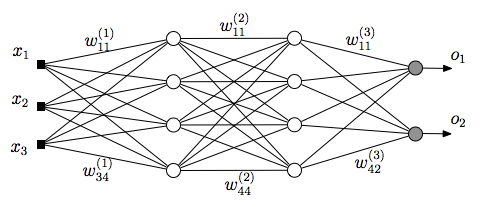
\includegraphics[scale=0.5]{img/MLP}
%    \caption{Paveikslėlio pavyzdys}
%    \label{img:mlp}
%\end{figure}


%\section{Eksperimentinio palyginimo rezultatai}
% tablesgenerator.com - converts calculators (e.g. excel) tables to LaTeX
%\begin{table}[H]\footnotesize
%  \centering
%  \caption{Lentelės pavyzdys}
%  {\begin{tabular}{|l|c|c|} \hline
%    Algoritmas & $\bar{x}$ & $\sigma^{2}$ \\
%    \hline
%    Algoritmas A  & 1.6335    & 0.5584       \\
%    Algoritmas B  & 1.7395    & 0.5647       \\
%    \hline
%  \end{tabular}}
%  \label{tab:table example}
%\end{table}

\end{document}
